\section{Analysis} 
\label{sec:analysis}

\noindent Consider the scalar linear system with equations of motion given by
the ODE
%
\begin{equation}
    m \ddot{x} + b\dot{x} + kx = u(x, \dot{x}),
    \label{eq:eom}
\end{equation}
%
where $u(x, \dot{x})$ is a control input that is to be determined for tracking.
We are uncertain of the constant parameters $\theta = \bmat{m & b & k}^\top$,
whose estimates are denoted by $\hat{\theta} \in \mathbb{R}^3$. Let us introduce
the errors in the position $x$, and parameters $\theta$ to be \[ \tilde{x} = x -
x_r, \quad \tilde{\theta} = \theta - \hat{\theta}, \quad e = \bmat{\tilde{x} &
\dot{\tilde{x}}}^\top, \] where $x_r$ is a reference
signal for the motion of the mechanical system. Inspired by Chapter 9
of~\cite{spong2020robot}, let us choose the control input according to 
\begin{align}
    \begin{split}
        u(x, \dot{x}) &= Y(x, \dot{x}, a, v)\hat{\theta} - cr, \\
        Y(x, \dot{x}, a, v) &= \bmat{a & v & x},
    \end{split}
    \label{eq:ctrl_law}
\end{align}
%
where the quantities $v$, $a$, and $r$ are given as
\begin{align*}
    v &= \dot{x}_r - \lambda \tilde{x}, \\
    a &= \dot{v} = \ddot{x}_r - \lambda \dot{\tilde{x}}, \\
    r &= \dot{x} - v = \dot{\tilde{x}} + \lambda \tilde{x},
\end{align*}
%
where $c, \lambda > 0$ are constant gains. Substituting the control
law~\eqref{eq:ctrl_law} into the system model~\eqref{eq:eom} leads to
%
\begin{equation}
    m\dot{r} + (b+c)r = -Y\tilde{\theta}.
    \label{eq:control_applied}
\end{equation}
%
The parameter estimate $\hat{\theta}$ may be computed using standard methods of
adaptive control such as gradients or least squares. For example, for a positive
definite matrix $\Gamma$ of appropriate dimensions, we can use the gradient
update law
%
\begin{equation}
    \dot{\hat{\theta}} = -\Gamma^{-1}Y^\top(x, \dot{x}, a, v)r.
    \label{eq:param_update}
\end{equation}

Consider the Lyapunov function candidate
%
\begin{equation*}
    V(\tilde{x}, \dot{\tilde{x}}, \tilde{\theta}) = \frac{1}{2}mr^2 + 
    c\lambda\tilde{x}^2 + \frac{1}{2}\tilde{\theta}^\top\Gamma\tilde{\theta}.
%     \label{eq:lyap_cand}
\end{equation*}
%
This is a positive definite function over the space of $\pmat{\tilde{x},
\dot{\tilde{x}}, \tilde{\theta}}$. We take the time derivative of the Lyapunov
function candidate and substitute from the closed-loop system
dynamics~(\ref{eq:control_applied}, \ref{eq:param_update}). We suppress its
functional dependence for brevity.
%
\begin{align}
    \begin{split}
    \dot{V} &= mr\dot{r} + 2c\lambda \tilde{x}\dot{\tilde{x}} +
    \tilde{\theta}^\top\Gamma\dot{\tilde{\theta}} \\
            &= r\left(-(b+c)r - Y\tilde{\theta}\right) + 2c\lambda
            \tilde{x}\dot{\tilde{x}} + \tilde{\theta}^\top Y^\top r \\
            &= -e^\top Qe \leq 0,
    \end{split}
    \label{eq:Vdot}
\end{align}
%
where $Q$ is a symmetric, positive-definite matrix given as \[ Q =
\bmat{(b+c)\lambda^2 & b\lambda \\ b\lambda & b+c}. \]
%
%
% Under some mild persistence of excitations conditions on $x_r(t)$, no
% solution can stay identically in $S$ other than the trivial solution
% $(\tilde{x}, \dot{\tilde{x}}, \tilde{\theta}) = (0,0,0)$. Therefore, invoking
% Corollary 4.1 of~\cite{khalil2015nonlinear} proves that all the errors converge
% to zero.~\todo{incorrect: not an autonomous system.}
% %
% Indeed, for any solution that belongs identically to $S$, the system
% dynamics yields \[ \tilde{m}\ddot{x}_r + \tilde{b}\dot{x}_r + \tilde{k}x_r
% \equiv 0, \qquad \dot{\tilde{m}} \equiv \dot{\tilde{b}} \equiv \dot{\tilde{k}}
% \equiv 0. \] 
%
Integrating both sides of equation~\eqref{eq:Vdot} gives \[ V(t) - V(0) =
-\int_0^t e^\top(\sigma) Q e(\sigma) \dd \sigma < \infty. \] We observe that
$\dot{\tilde{x}}$ is bounded because $\dot{V} \leq 0$ implies that the terms
$r$, $\tilde{x}$ and $\tilde{\theta}$ are bounded functions of time. This allows
us to invoke Barbalat's lemma~\cite{spong2020robot} to deduce that $\tilde{x}
\rightarrow 0$ as $t \rightarrow \infty$. Furthermore, using
equation~\eqref{eq:control_applied}, we can readily see that $\ddot{x}$ is
bounded. Another application of Barbalat's lemma shows that the velocity error
$\dot{\tilde{x}} \rightarrow 0$ provided that the reference acceleration
$\ddot{x}_r(t)$ is bounded. Since $x \rightarrow x_r$, we also have that $u(x,
\dot{x}) \rightarrow \hat{m}\ddot{x}_r + \hat{b}\dot{x}_r + \hat{k}x_r$.

\begin{figure}[h!]
  \centering
  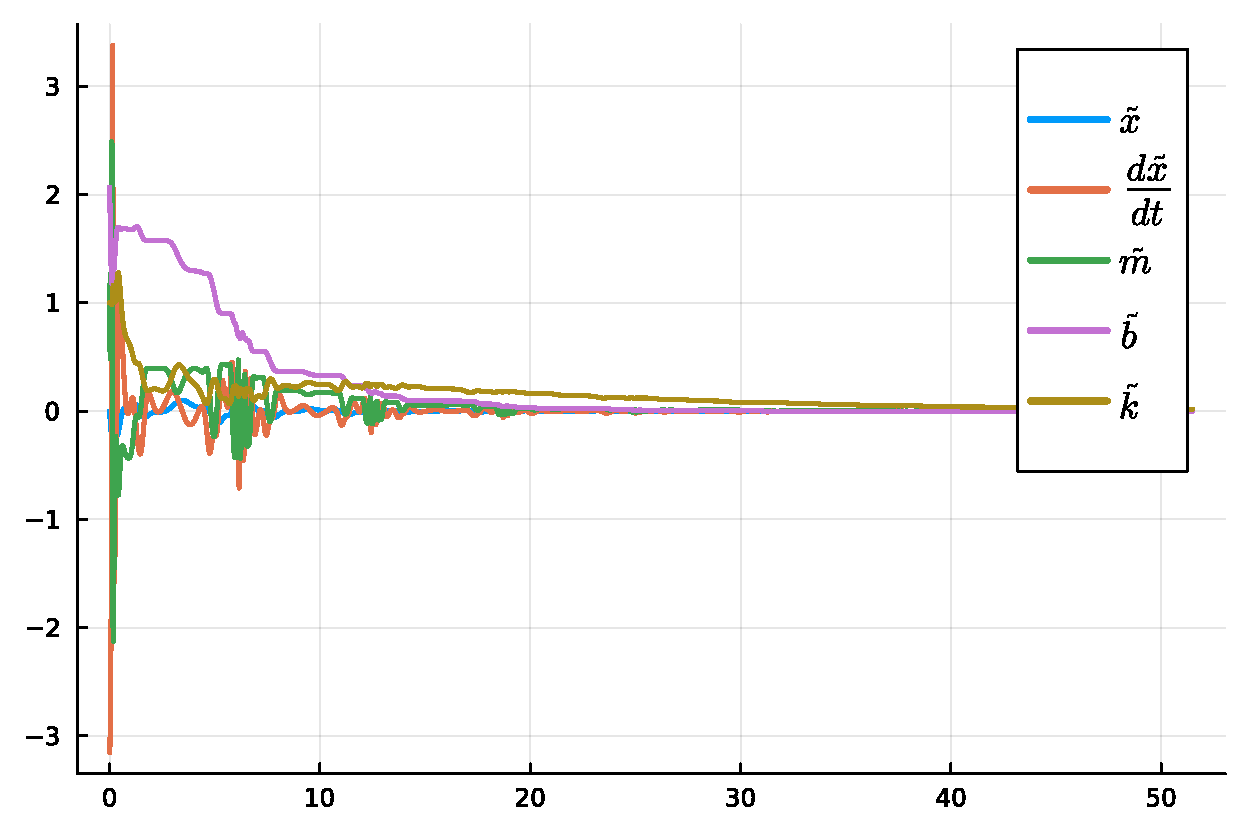
\includegraphics[width=0.75\textwidth]{./figures/adaptationrule2.pdf}
  \caption{Simulation showing the convergence of the system state and parameter
  estimates.}
  \label{fig:adaptation}
\end{figure}

For any $\eta > 0$, the set $\Omega_\eta = \{(e, \tilde{\theta}): V(\tilde{x},
\dot{\tilde{x}}, \tilde{\theta}) \leq \eta\}$ is positively invariant. The
positive limit set of $(e(t),\tilde{\theta}(t))$ is a subset of $E = \{(e,
\tilde{\theta}): e = 0\}$. Unfortunately, for a general nonautonomous system,
the positive limit set is not necessarily a positively invariant set, precluding
us to invoke LaSalle's theorem to conclude that $\tilde{\theta} \rightarrow
0$~\cite{khalil2015nonlinear}.

%
We can excite several frequencies by choosing 
\begin{align*}
    x_r(t) &= A\sin{\left(\omega(t) + \varphi\right)} \\
    \omega(t) &= \pi\sum_{k=1}^n \left(1-\frac{k-1}{n}\right)\sin{k t}
\end{align*}
%
for some constants $\varphi$, $A > 0$, and a sufficiently large $n \in
\mathbb{N}$. Simulation results in the next section suggests that this coaxes
$\tilde{\theta} \rightarrow 0$ even though we were only able to show that
$\tilde{\theta}$ is bounded in theory. 
% making the origin of $(\tilde{x},
% \dot{\tilde{x}}, \tilde{\theta})$ globally asymptotically stable.
